%goals
Our project is intended to manipulate image frames in a video of a model hand demonstrating nail polish product so that the model hand takes on the user's skin colour. The images we must process will mostly consist of the back of a single hand shown prominently in the image. We expect image sizes the algorithm should be able to handle to be relatively large, at least approximately 800 by 800 pixels in size. We show an example of the desired output of our algorithm in Table \ref{tab:our_demo}.

\begin{table}[H]
	\centering
	\caption{Example of our desired output given a source (the model) and a target image (from the user) \label{tab:our_demo}}	
\begin{tabular}{|c|c|c|}
	\hline
	Source & Target & Output \\ 
	\hline
	  \begin{minipage}{.29\textwidth}
	    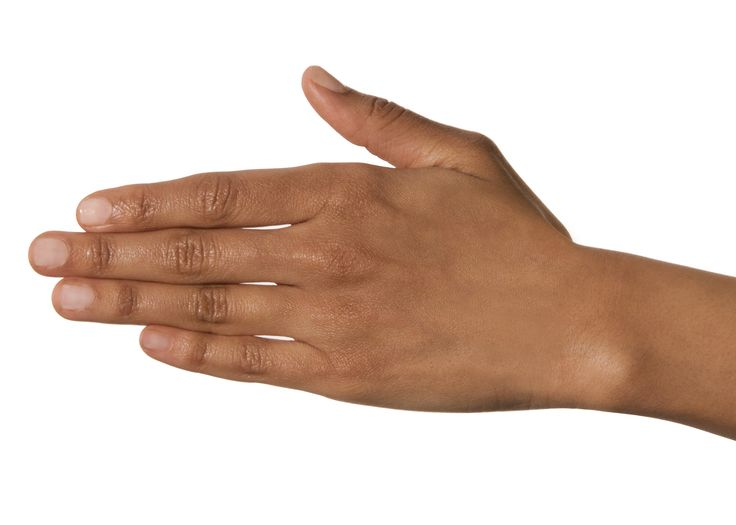
\includegraphics[width=\textwidth,height=\textheight,keepaspectratio]{../inputs/hand_brown.jpg}
	  \end{minipage} & 
	  \begin{minipage}{.29\textwidth}
	    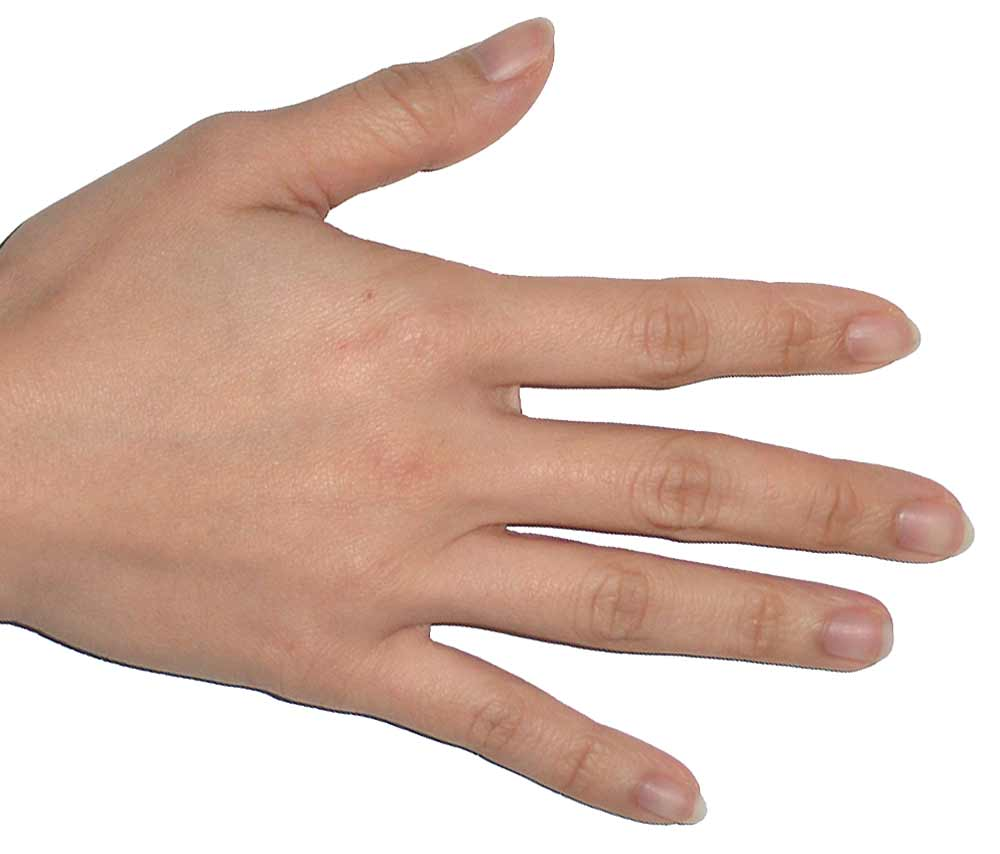
\includegraphics[width=\textwidth,height=\textheight,keepaspectratio]{../inputs/hand_light.jpg}
	  \end{minipage} & 
	  \begin{minipage}{.29\textwidth}
	    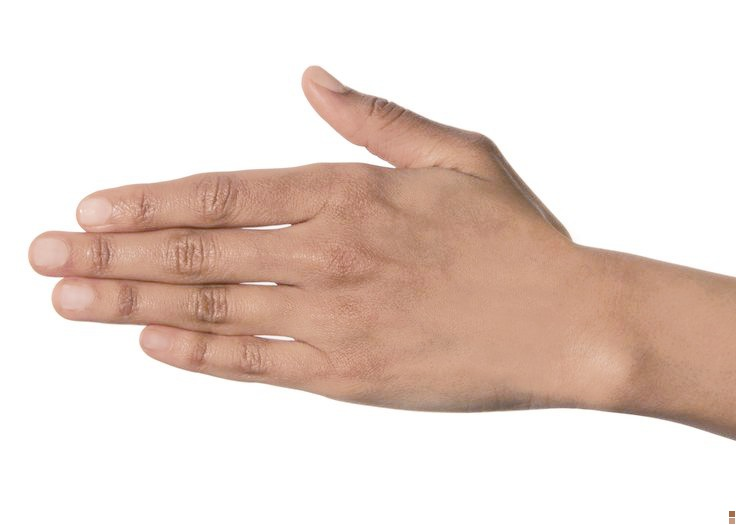
\includegraphics[width=\textwidth,height=\textheight,keepaspectratio]{../rc_test/outputs/20170524_prop_corr_1p1_ave_100/hand_brown_to_hand_light.jpg}
	  \end{minipage} \\
	\hline
 \end{tabular}
 \end{table}

To narrow the scope of our project, we will not include skin detection as part of this project and assume that our algorithm is already given a mask of the skin areas of all the images. We will focus solely on the transfer of the hand skin colour. 

Based on our goals and the nature of our project, we list below several constraints and design paradigms for our algorithm:

\textbf{Compatible with mobile device:} Our algorithm is ultimately intended to support an application on a mobile device, so we must ensure that our code is easily portable to mobile platforms and that the algorithm we develop can operate quickly with the limited resources of a mobile device so that the user will be able to see near-instant results.

\textbf{Fully automatic:} Since the goal of our project is for a commercial user to be able to easily adjust the model image to have his or her own skin colour, our algorithm cannot rely on any user input to perform the image editing and should be only require an image containing the user's own hand as the target image for performing the colour transfer on the model.

\textbf{Realistic skin colour transfer:}
Since the results of the algorithm are meant to invoke for the user the impression that the user's own hand is wearing a cosmetic product, and since we can expect that the user would be sensitive to both an image of their own hand and the subtle effect of a particular cosmetic product, our final images must look as realistic as possible to avoid displeasing, uncanny valley effects. Furthermore, the images we process will be large and feature the skin on the back of a hand very prominently, so we can expect that unrealistic flaws in our result will be very noticeable the user.

\textbf{Accurate skin colour transfer:} 
Since the purpose of the nail polish try-on application is to demonstrate to the user how a particular shade of nail polish will appear on the user's own hand, we must ensure that the results of the algorithm, more than looking pleasing to the user, actually matches the skin colour sample provided by the user so as to give the user a realistic preview of the product.

\textbf{Wide range of colour transfer:} Since the project is motivated by the goal to support users with a wide range of skin colours while avoiding the necessity of manually creating a large number of nail polish try-on videos of different skin colours, our algorithm needs to be able to transfer the skin colour of a mid-toned hand to as wide a range of skin colour as possible.